\chapter{Despacho Ótimo no Tempo}
\localtableofcontents 

Este capítulo é baseado nas notas de aula do curso, ministrado em 10/08/2023, e nas informações do Capítulo~7 de \textcite{cretì_fontini_2019}.

\section{Fundamentos}
Alguns conceitos serão fundamentais para o compreendimento da dimensão temporal do consumo de eletricidade. O primeiro deles é o de fator de capacidade (\textit{Capacity Factor}), já o segundo é a duração de carga (\textit{Load Duration}).
\begin{defin}[Fator de Capacidade]
    A fração de uma quantidade total de tempo em que existe uma determinada quantidade de carga ou geração sobre o sistema.
\end{defin}
\begin{defin}[Duração de Carga]
    O inverso da função de densidade acumulada da carga em relação ao fator de capacidade em um intervalo de tempo específico.
\end{defin}
Naturalmente, ambos conceitos estão intrinsecamente ligados. Tome, por exemplo, a Figura~\ref{fig:carga}, na qual está exemplificada a carga horária sobre o sistema ao longo de um ano inteiro. Se fosse de interesse exprimir a proporção do tempo em que o sistema está sobre determinado nível de carga, chegaríamos então na Figura~\ref{fig:load}.

\begin{figure}[t]
    \centering
    \begin{subfigure}{\textwidth}
        \centering
        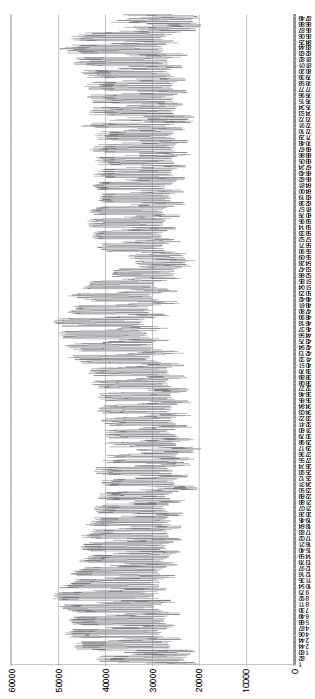
\includegraphics[scale=.5,angle=-90]{figure/carga.png}
        \caption{Exemplo de carga horária sobre o sistema}
        \label{fig:carga}
    \end{subfigure}\\
    \begin{subfigure}{\textwidth}
        \centering
        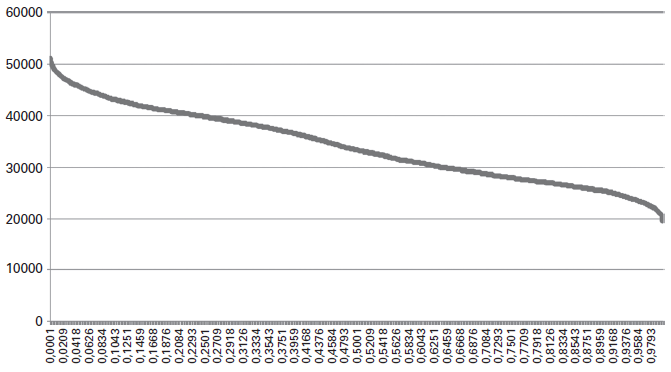
\includegraphics[scale=.5]{figure/load.png}
        \caption{Duração de Carga}
        \label{fig:load}
    \end{subfigure}
    \caption{Relação entre Duração de Carga e Fator de Capacidade}
    \subcaption*{\footnotesize \textit{Nota:} O eixo vertical de ambas figuras representa o total de carga em MWh sobre o sistema. No Painel (a) o eixo horizontal representa as horas do ano, já no Painel (b) representa o fator de capacidade}
\end{figure}  

Da definição a duração de carga temos a ideia de probabilidade - ou densidade acumulada. Esse conceito é importante, pois é uma das principais formas de como ler a Figura~\ref{fig:load}. De forma analítica, temos que: 
\[F(cf) = \{\omega | P(X\leq \omega) = cf\}\]
onde $F(\cdot)$ é a função duração de carga, $X$ é uma variável aleatória representativa da carga sobre o sistema e $cf$ é o fator de capacidade.

\section{Propriedades da Função Custo}
Considere a seguinte forma simplificada de uma função custo (total), onde há uma componente de custo fixo ($FC_i$) e outra de custo variável ($c_i'q_i$):
\[c_i(q_i)=FC_i+c_i'q_i\]

Suponha que ela exprima o custo por hora. Ademais, suponha que a usina $i$, cuja capacidade (por hora) é $q_i^{max}$, produz um total de energia por ano $yq_i = q_i^{max}\cdot h_i$, onde $0\le h_i\le8760$. Ora, repare que $h_i$ denota o a quantidade de tempo efetiva durante a qual a usina $i$ está produzindo ao longo do ano, o que pode ser expresso em termos de fator de capacidade como $h_i=cf_i\cdot8790$. Finalmente, suponha que $FC_i=hRC_i\cdot q_i^{max}$, onde $hRC_i$ denota o custo de aluguel por hora da usina $i$. Podemos, então, reescrever a função acima como:
\[yc_i(q_i)=hRC_i\cdot q_i^{max}\cdot8760+c_i'\cdot q_i^{max}\cdot cf_i\cdot8760\]

Seguem duas definições importantes para o argumento dos próximos capítulos:
\begin{defin}[Custo Médio de Energia - CME]
    O custo de geração por unidade de energia produzida ou produzível.
\end{defin}
Neste exemplo acima, é imediato calcular o CME:
\[CME \equiv \frac{yc_i}{yq_i} = \frac{hRC_i}{cf_i}+c_i'\]
\begin{defin}[Custo Médio de Capacidade - CMC]
    O custo de geração por unidade de capacidade instalada ou instalável.
\end{defin}
Da mesma forma, o CMC é dado por:
\[CMC\equiv \frac{yc_i}{q_i^{max}\cdot8790} = hRC_i+c_i'\cdot cf_i\]
Uma representação gráfica para a equação acima é dada na Figura~\ref{fig:cmc}, considerando $c_i'=\alpha$ e $hRC_i=FC_3$, por exemplo.
\begin{figure}[t]
    \centering
    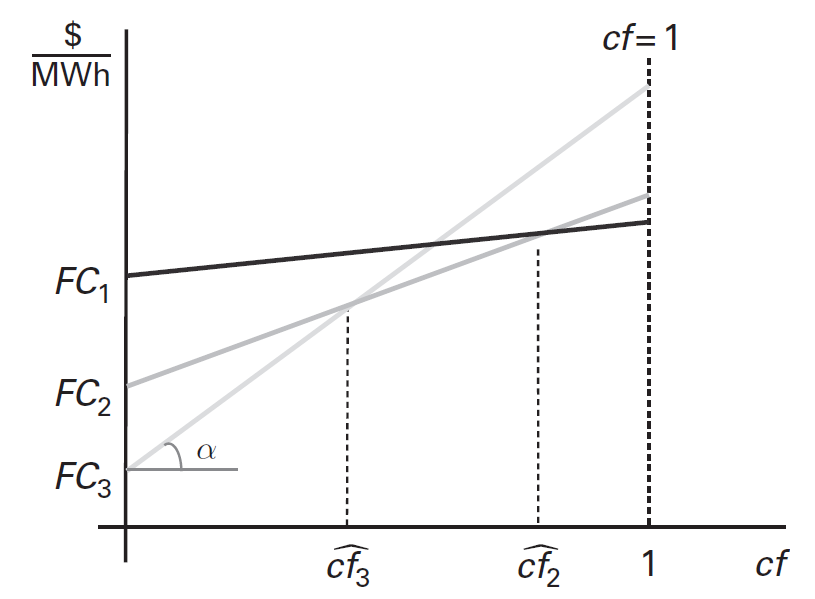
\includegraphics[scale=.3]{figure/cmc.png}
    \caption{Custo Médio de Capacidade - CMC}
    \label{fig:cmc}
\end{figure}

\section{Problema do Planejador Central em T Horas}
Podemos pensar a dimensão temporal do problema a partir dos dados. Lembre que a cuva de Duração de Carga pode ser interpretada como a probabilidade de se encontrar um determinado valor $\overline{Q}$ - associada à um fator de capacidade. Portanto, podemos pensar que um problema estático é resolvido em cada instante de tempo e, destarte, é natural inferir que em uma estrutura energética que atende à ordem de mérito o número em operação vai depender do fator de capacidade de cada instante $t$. É isso o que vamos discutir nessa seção.

De forma geral, podemos ligar vários dos conceitos que vimos até agora tal qual exposto na Figura~\ref{fig:welfare_time}. Nela, supomos um sistema representado pela curva de Duração de Carga descrita no canto direito superior da figura. Note que o sistema sempre utiliza ao menos $M^{min}$ e, em contrapartida, opera com no máximo $M^{max}$. Supomos também que existem apenas três usinas - $A$, $B$ e $C$ - e que o custo marginal é crescente por usina, mas que o oposto vale para os custos fixos ($FC_i$). A solução do problema de maximização do bem-estar que segue a ordem de mérito fornecido pelos custos marginais também é chamado de despacho econômico.

\begin{figure}
    \centering
    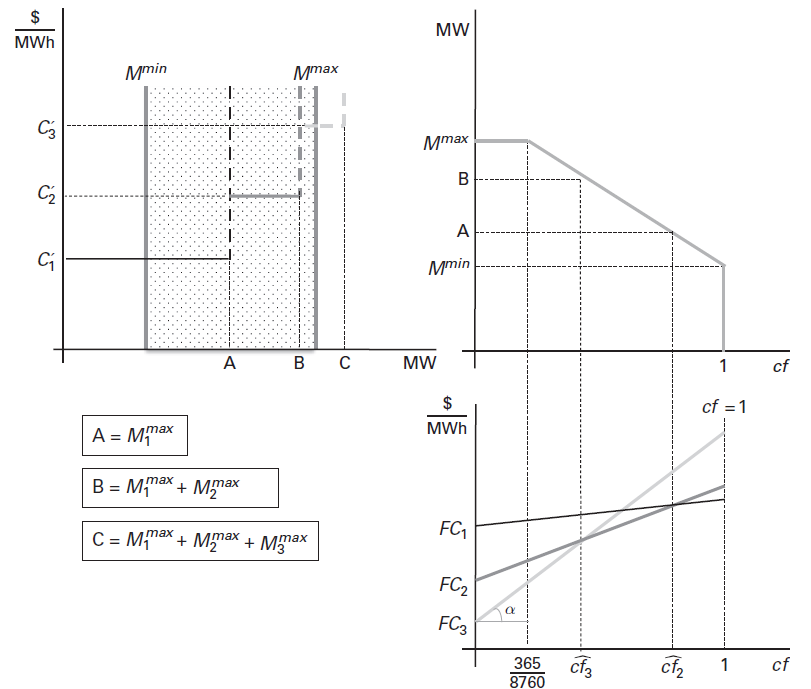
\includegraphics[scale=.5]{figure/economic_dispatch.png}
    \caption{Problema de Maximização de Bem-Estar ao Longo do Tempo}
    \label{fig:welfare_time}
\end{figure}

\begin{defin}[Despacho Econômico]
    A utilização/ativação das usinas é feito de acordo com a ordem de mérito fornecida pelos custos marginais.
\end{defin}

Note que, seguindo o despacho econômico, quando a carga está no mínimo apenas a planta $A$ é acionada. Isso muda exatamente no ponto em que a carga é tal que a usina $A$ não é capaz de suprir a demanda energética ou, alternativamente, em que o fator de capacidade implica o CMC da próxima unidade de eletricidade ser menor na usina $B$ que na usina $A$. 

Mais ainda, repare que a área entre o intervalo de carga gerado (no máximo) por uma usina e o eixo horizontal equivale ao total de energia gerado por ela - tal qual exemplificado na Figura~\ref{fig:tot_energy}. Mais ainda, a energia (potencialmente) gerada pela usina de menor custo marginal é denominada \textbf{carga base} (\textit{base load}), euqnato a energia grada pela usina menos eficiente é denominada \textbf{carga de pico} (\textit{peak load}). A energia gerada entre a carga base e carga de pico é denominada, por sua vez, de \textit{mid-merit}.

\begin{figure}
    \centering
    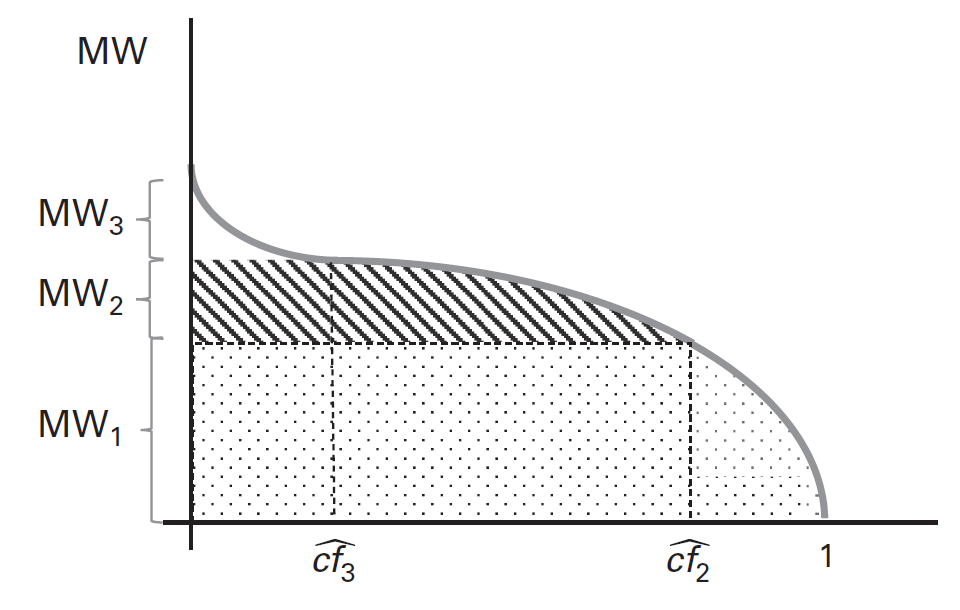
\includegraphics[scale=.25]{figure/tot_energy.png}
    \caption{Total de Eletricidade Gerado por Usina}
    \label{fig:tot_energy}
\end{figure}

\section{Desligamento de Carga Otimizado}
Note que no exemplo descrito na subseção anterior é assumido $M^{max}<A+B+C$ i.e. que a capacidade de geração é maior que a carga máxima do sistema - hipótese que flexibilizaremos aqui. 

Para responder o que acontece nesse caso de claro desiquilíbrio, lembre do Problema do Planejador Central descrito na seção anterior e da simetria de seus resultados com o Problema do Monopolista. Visto que a teoria é perfeitamente análoga, podemos demonstrar que existirá uma "ordem de mérito" para consumidores também, ordenados por suas utilidades marginais. Destarte, consumidores com maior utilidade marginal serão supridos primeiro, seguindo a "ordem de mérito" sucessivamente.

Enquanto a carga for compatível com a capacidade do sistema é trivial observar que todos os consumidores serão atendidos. Entretanto, quando chegamos na carga de pico e, potencialmente, na carga máxima, suposta a partir de agora $M^{max}>A+B+C$, alguém deverá deixar de ser atendido. Resta, portanto, a pergunta sobre como determinar esse processo de forma a maximizar bem-estar. Ora, isso é facilmente respondido, novamente, pelo Problema do Planejador Central. Fixe um instante $t$ de tempo e suponha que neste instante a carga total demandada $\sum_nq^n\equiv Q^N$ é maior que a capacidade do sistema. O problema pode ser escrito como:
\begin{align*}
    \max_{Q^N\in\mathbb{R}}&\quad U(Q^N) - \sum_{i=1}^Ic_i(q_i)\\
    \text{s.a}&\quad Q^N=\sum_iq_i\\
    &\quad 0\le q_i \le q_i^{max},\quad \forall i=1,\hdots,I\\
    &\quad 0\le Q^N \le Q^{{N^{max}}}\equiv M^{max}\\
    &\quad M^{{N^{max}}}>\sum_iq_i^{max}
\end{align*}
Implicando Lagrangiano:
\begin{align*}
    \mathcal{L}=\sum_{i=1}^Ic_i(q_i)-U(Q^N)+\mu(Q^N-\sum_iq_i)+\lambda(\sum_iq_i^{max}-M^{{N^{max}}})
\end{align*}
Implicando a seguinte restrição de estacionariedade:
\begin{align*}
    \frac{\partial\mathcal{L}}{\partial Q^N} = -U'(Q^N) + \mu - \lambda = 0
\end{align*}
Ora, como a restrição referente à $\lambda$ é inativa, por definição, temos que $\lambda=0$, implicando $U'(Q^N) = \mu $. Seja $Q^{N^*}\equiv \Tilde{M}$ a solução do problema acima. A carga desligada (não servida) ótima pode ser escrita, portanto, como $M^{max}-\Tilde{M}$. Segue uma importante definição:
\begin{defin}[Valor da Carga Perdida - \textit{Value of Lost Load}, VOLL]
    O valor da carga referente a se ter uma unidade marginal a mais de capacidade instalada no sistema. 
\end{defin}
Note que o VOLL indica o valor que o consumidor está disposto a pagar para ter uma unidade a mais de energia i.e. o VOLL é expresso como $\mu$ no problema descrito acima (ver Capítulo~\ref{kkt}). Seguem mais duas definições importantes:
\begin{defin}[Expectativa de Carga Perdida, \textit{Loss of Load Expectation}, LOLE]
    O número de unidades de tempo em um dado período (por exemplo, horas do ano) em que se espera que a carga seja perdida.
\end{defin}
\begin{defin}[Probabilidade de Perda de Carga, \textit{Loss of Load Probability}, LOLP]
    A probabilidade de que em um determinado momento haverá perda de carga.
\end{defin}
Ora, se essa carga perdida representa um custo-oportunidade para os consumidores, ela pode ser expressa em unidades monetárias. Portanto, é possível recuperar uma "função dano" ($DF$) quantificando o valor econômico da expectativa de energia não servida:
\begin{align*}
    DF= LOLE\cdot \left(M^{max}-\Tilde{M}\right) \cdot VOLL 
\end{align*}

A Figura~\ref{fig:shedding} indica a interação dessa função dano com o equilíbrio discutido anteriormente. Note que no momento em que fator de capacidade é tal que o valor econômico da expectativa de energia não servida de uma unidade a mais de eletricidade é menor que o custo de produzi-la, cessa-se a geração de energia (ao nível $\Tilde{M}<M^{max}$).    

\begin{figure}
    \centering
    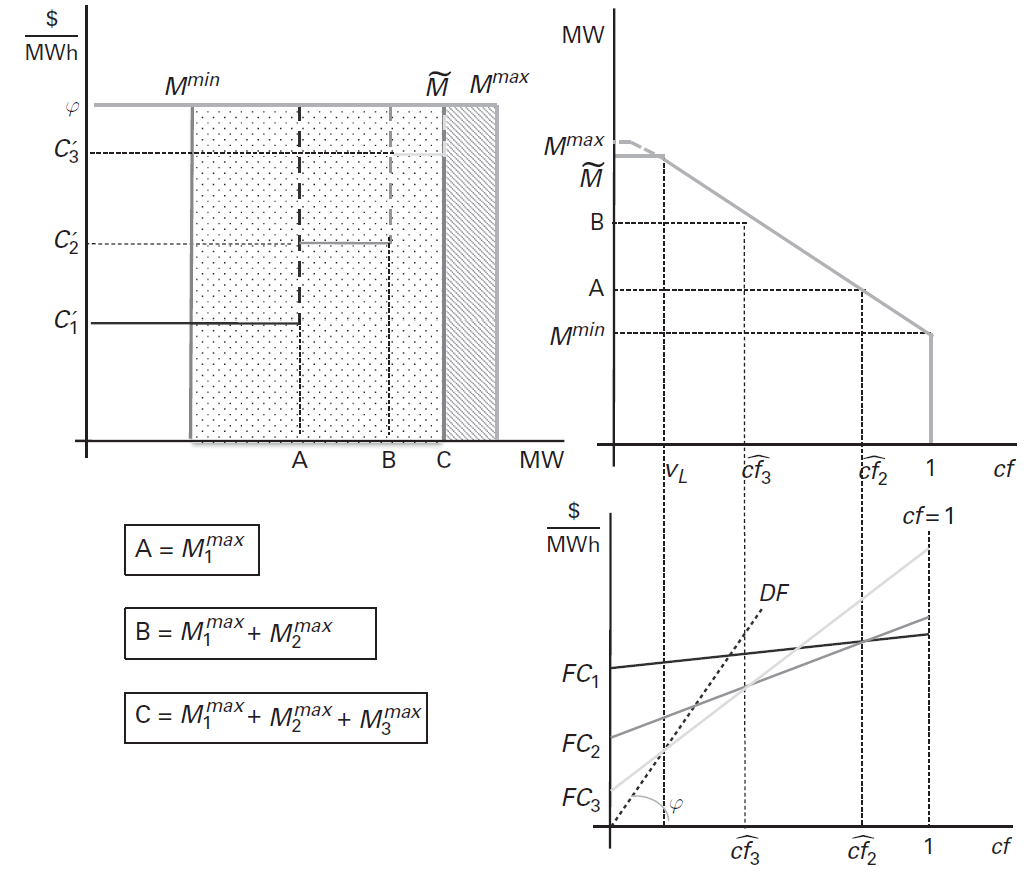
\includegraphics[scale=.4]{figure/shedding.png}
    \caption{Problema de Maximização de Bem-Estar ao Longo do Tempo com Desligamento de Carga}
    \label{fig:shedding}
\end{figure}
